%%%%%%%%%%%%%%%%%%%%%%%%%%%%%%%%%%%%%%%%%%%%%%%%%%%%%%%%%%%%%%%%
% Sim
%%%%%%%%%%%%%%%%%%%%%%%%%%%%%%%%%%%%%%%%%%%%%%%%%%%%%%%%%%%%%%%%
\section{仿真}
本文使用基于C++的仿真器\cite{olzhn2021}进行仿真。

% ////////////////////////////////////////
\subsection{给定参数计算}
给定出发点和到达点的改进春分点轨道根数分别为
\begin{center}\begin{tabular}{lll}
    \toprule
    名称 & 出发点 & 到达点 \\
    \midrule
    p & $1.00056767075005     $ & $1.51037523709971    $ \\
    f & $-0.00294437794279988 $ & $0.0854235624895203  $ \\
    g & $0.0162420106027165   $ & $-0.0378544516020575 $ \\
    h & $1.06259234267730e-05 $ & $0.0104735801650767  $ \\
    k & $3.28399488220299e-07 $ & $0.0122796628620782  $ \\
    L & $2.43306352346982     $ & $5.76521463465294    $ \\
    \bottomrule
\end{tabular}\end{center}
计算可得开普勒轨道根数为
\begin{center}\begin{tabular}{lll}
    \toprule
    名称 & 地球 & 火星 \\
    \midrule
    半长轴    a & $ 1.000840$ & $ 1.523677$ \\
    偏心率    e & $ 0.016507$ & $ 0.093435$ \\
    轨道倾角  i & $ 0.000021$ & $ 0.032276$ \\
    升交点赤经Ω & $ 0.030896$ & $ 0.864609$ \\
    近地点幅角ω & $-1.422358$ & $-1.281742$ \\
    真近点角    & $ 3.824526$ & $ 6.182348$ \\
    $\mu$值     & $398601   $ & $42808    $ \\
    \bottomrule
\end{tabular}\end{center}
另,太阳$\mu$值为$\mu_s=132706538114$。
其它设定参数为
\begin{center}\begin{tabular}{ll}
    \toprule
    名称 & 值 \\
    \midrule
    航天器质量 & 1000kg \\
    推力 & 1N \\
    比冲 & 2000s \\
    转移时间 & 260天 \\
    \bottomrule
\end{tabular}\end{center}
可算出以速度为单位的比冲为$I_{sp}=19600$m/s,
也就是说保持发动机推力$F=1$N时,
燃料消耗速度为$d_m=1/19600$千克/秒,
限制发动机工作时间不超过$T_f=19600*400=7.84\times10^6$秒,约90天。
为统一单位,将长度单位全部换算成km,
则推力为$F=10^{-3}$kN。
另外考虑单位换算,
燃料消耗速度$d_m$和推力$F$的换算关系为
\begin{align*}
    &\bar{d}_m\left[\frac{\text{kg}}{10^{-4}\text{s}}\right]
    = 10^4d_m\left[\frac{\text{kg}}{\text{s}}\right] \\
    &\bar{F}\left[\frac{\text{kg}\cdot(10^{-6}\text{km})}{(10^{-4}\text{s})^2}\right]
    = 10^2F\left[\frac{\text{kg}\cdot\text{km}}{\text{s}^2}\right] \\
\end{align*}

% ////////////////////////////////////////
\subsection{建模}
假设探测器在转移轨道上不受地球和火星引力影响。
考虑燃料消耗的火星探测器动力学方程为
\begin{align*}
    &\ddot{\vec{r}} = -\frac{\mu_s}{||\vec{r}||^3}\vec{r}
    + \frac{10^{-3}}{m(t)}\epsilon(t)
    \left[\begin{matrix}
        \cos\phi\cos\theta \\ \cos\phi\sin\theta \\ \sin\phi
    \end{matrix}\right] \\
    &\dot{m}(t) = -\frac{1}{19600}\epsilon(t)
\end{align*}
其中
$\phi$和$\theta$分别为发动机推力向量的俯仰角和方位角,
$\epsilon(t)=0$或$1$表示发动机开机或关机。
建立探测器器被控对象模型的模块框图如图\ref{figSimPlant}所示。
\begin{center}
	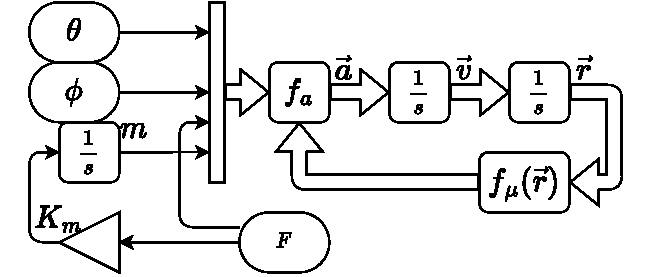
\includegraphics[scale=0.8]{plant.pdf}  \\
	\figcaption{火星探测器被控对象模型的模块框图}\label{figSimPlant}
\end{center}
其中$K_m=-\frac{\bar{d}_m}{F}$。

% ////////////////////////////////////////
\subsection{仿真调试}
为了验证建模与仿真结果正确,
将部分调试步骤和中间结果记录如下。

\noindent\textbf{绘制轨道}\par
为验证出发点与到达点结果正确,
分别从出发点与到达点开始绘制半个公转周期轨道作为参考,如图\ref{figSimDebug1}所示。
\begin{center}
	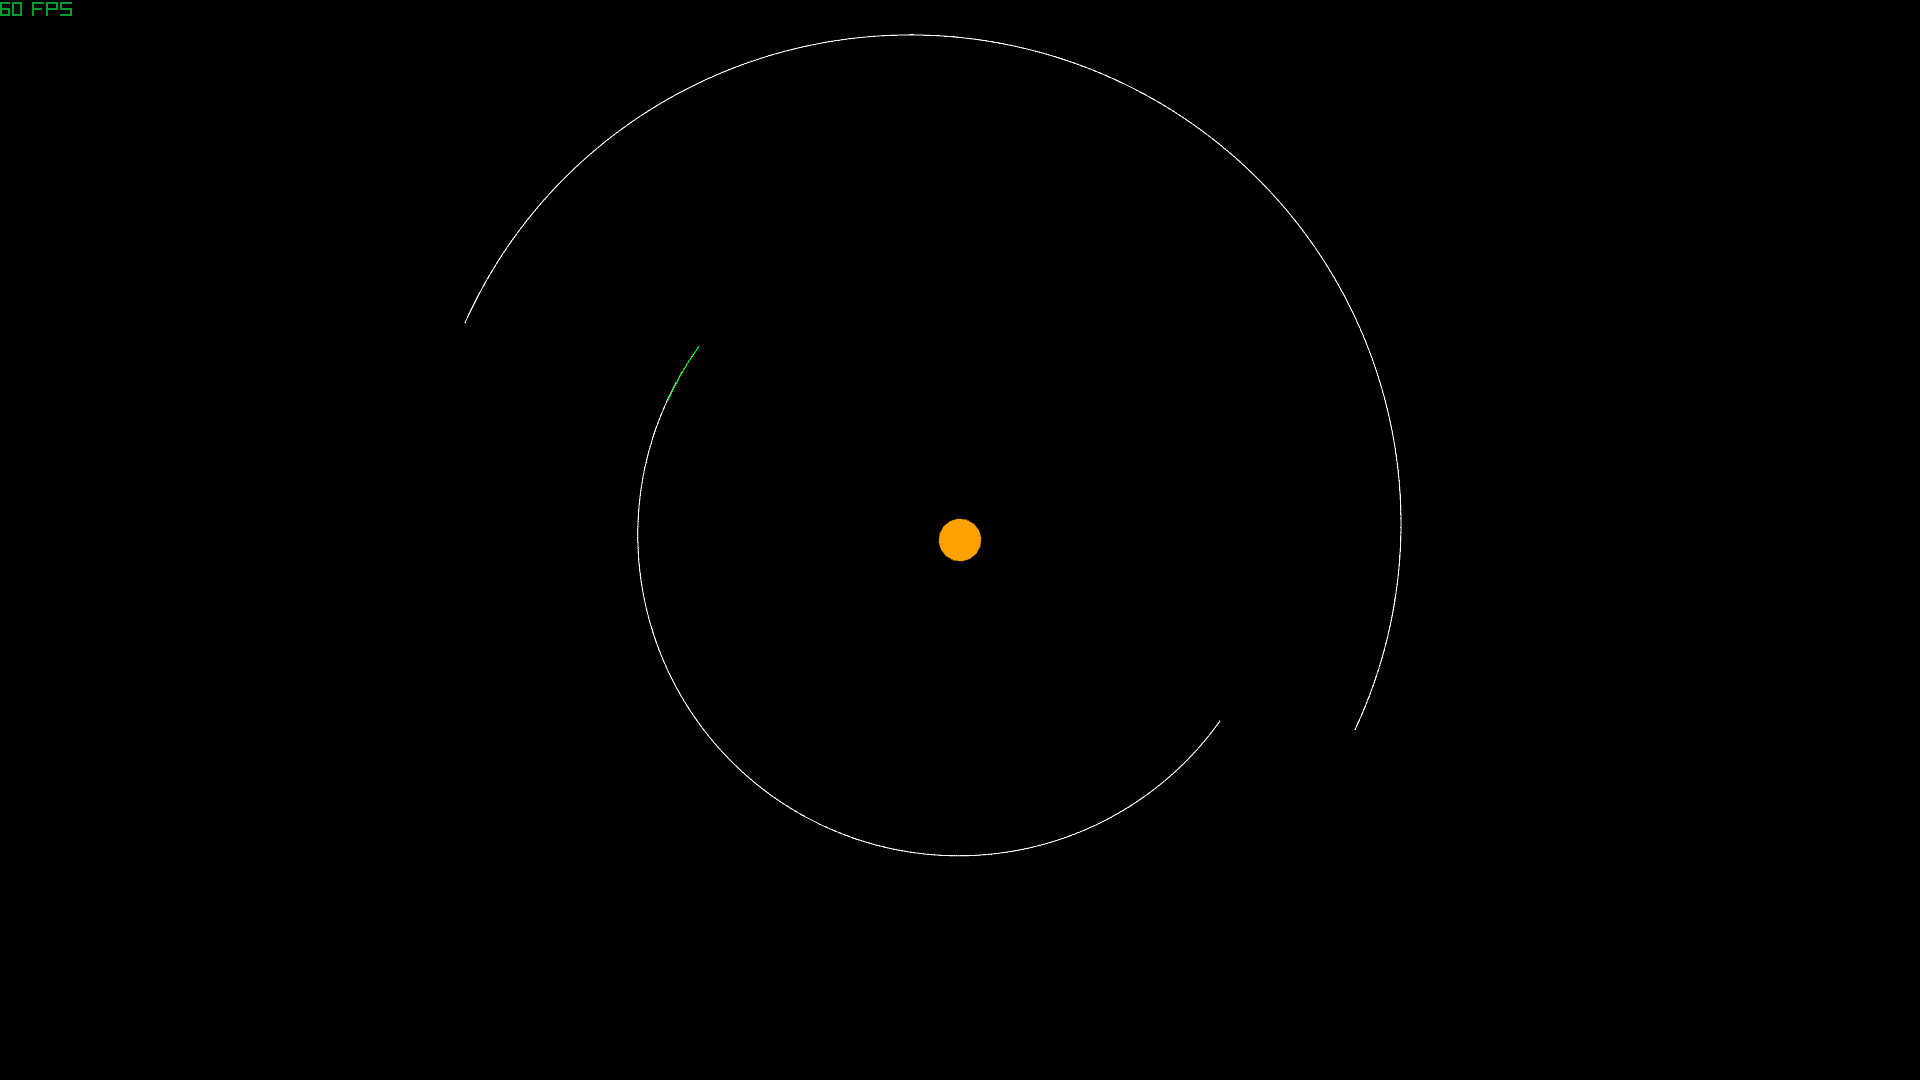
\includegraphics[scale=0.2]{simdebug1.png}  \\
	\figcaption{地球和火星的半个公转周期轨道俯视图}\label{figSimDebug1}
\end{center}
地球和火星的公转周期分别按365天和687天计算,
半个公转周期分别为$1577$和$2968$仿真器秒。
1仿真器秒等于$1000$仿真步长,
1仿真步长等于实际时间10秒。
仿真器坐标下的出发点位置和速度向量分别为
\[[\begin{matrix}
    -113.102 & 101.033 & 0.00219
\end{matrix}]\]
\[[\begin{matrix}
    -0.19353 & -0.22118 & -4.517067e-06
\end{matrix}]\]
结果基本正确。

\noindent\textbf{燃料消耗}\par
仿真$10^5$个步长后,
仿真得剩余总质量为$948.98$kg。
$10^5$个步长对应$10^6$秒,
燃料消耗$10^6\times\frac{1}{19600}=51.02$kg,
结果正确。
图\ref{figSimDebug1}中的绿色轨迹为
发动机推力俯仰角为0,方位角为$-1.57$时持续工作$10^5$个步长的结果。
